\documentclass[a4paper,12pt]{article}

%\begin{figure}[htp]
%    \centering
%    \includegraphics[width=0.75\textwidth]{}
%\end{figure}

%%%%%%%%%%%%%%%%%%%%
%%%%  PREAMBLE  %%%%
%%%%%%%%%%%%%%%%%%%%
\usepackage{float}
\usepackage[T1]{fontenc}
\usepackage[utf8]{inputenc}

\usepackage[english,italian]{babel}
\usepackage{graphicx}     % Per includere immagini
\usepackage{subcaption}   % Per utilizzare subfigure
\usepackage{hyperref}
\usepackage{indentfirst}

\hypersetup{hidelinks}

\usepackage[margin=2.5cm]{geometry}
\usepackage{minipage-marginpar}
\usepackage{fancyhdr}
\usepackage[bottom]{footmisc}
\usepackage{lastpage}

\usepackage{enumitem}
\usepackage{tabularx}

\usepackage{graphicx}

\setlength{\parindent}{0em}
\setlength{\parskip}{1em}

\fancyhead[L]{\leftmark}
\fancyhead[R]{\shortstack[r]{Versione documento: 0.01 \\ Gruppo: G24}}

\fancyfoot[C]{}
\fancyfoot[R]{\thepage/\pageref{LastPage}}

\renewcommand{\headrulewidth}{2pt}
\renewcommand{\headruleskip}{3pt}
\setlength{\headheight}{30pt}

\renewcommand{\footrulewidth}{2pt}

\setlist[itemize]{itemsep=0.25em,topsep=0pt}
\setlist[enumerate]{itemsep=0.25em,topsep=0pt,align=left}

%%%%%%%%%%%%%%%%%%%%
%%%%  DOCUMENT  %%%%
%%%%%%%%%%%%%%%%%%%%

\title{}
\author{Gruppo G24}

\begin{document}

\pagestyle{empty}

\begin{center}

    \vspace{2 cm}

    \begin{tabular*}{\textwidth}{ c @{\extracolsep{\fill}} c }
        
\includegraphics[width=0.3\textwidth]{marchio_unitrento.pdf} & \shortstack{\Large{Dipartimento di Ingegneria} \\ \Large{e Scienza dell'Informazione}}
    \end{tabular*}

    \vspace{5 cm} 
  
    \Huge \textbf{Ingegneria del software\\}
  
    \vspace{1.5 cm} 
    \Large\textsc{Documento dei requisiti\\} 
    \vspace{3 cm} 
    \Huge\textsc{Mountain Wonders\\}
    \Large{Gruppo G24}
  
    \vspace{2 cm} 
  
    \Large{Anno accademico 2023/2024}
\end{center}

\newpage
\tableofcontents

\pagestyle{fancy}
\newpage
\section{Scopo del documento}

Il presente documento riporta la specifica dei requisiti di sistema del progetto MountainWonders. Lo scopo di questo documento è quello di mostrare le specifiche dei requisiti funzionali e non funzionali tramite l'utilizzo di diagrammi UML (Unified Modeling Language), diagrammi degli use-case, tabelle, context diagram e component diagram.\\
All'interno del documento precedentemente consegnato, sono stati specificati i requisiti funzionali e non funzionali in linguaggio naturale, mentre ora verranno espressi utilizzando un linguaggio più formale e strutturato.
    
\newpage

\section{Requisiti funzionali}

Vengono elencati di seguito i requisiti funzionali(RF) dell'applicazione, tramite l'utilizzo degli Use Case Diagram.

\subsection*{RF5 Account anonimo}

\subsubsection*{RF1 Registrazione}
\begin{figure}[H]
   \centering
    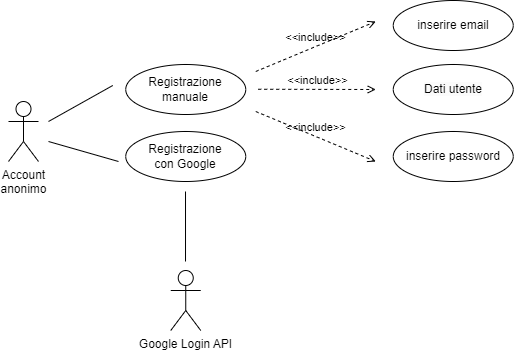
\includegraphics[width=0.8\textwidth]{img-D2/registrazione_anonimo.png}
    \caption{USE-CASE Registrazione}
\end{figure}

\begin{figure}[H]
   \centering
    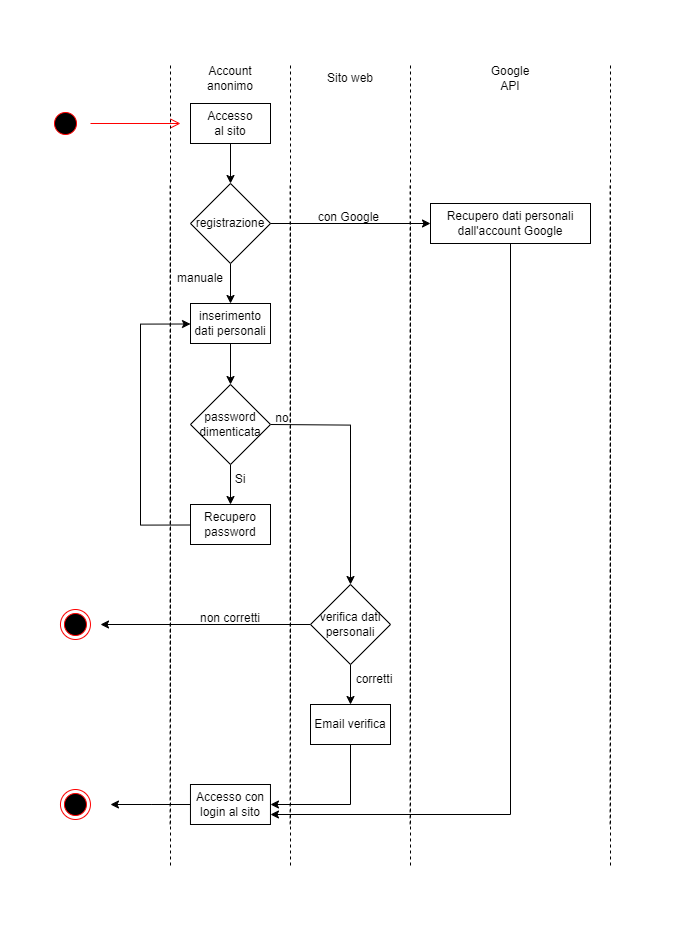
\includegraphics[width=1\textwidth]{img-D2/diagramma_registrazione.png}
    \caption{Diagramma attività registrazione}
\end{figure}


\subsubsection*{RF2 Login}
\begin{figure}[H]
   \centering
   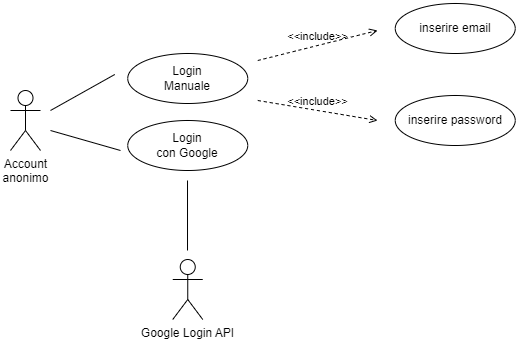
\includegraphics[width=0.8\textwidth]{img-D2/login_anonimo.png}
    \caption{USE-CASE Login}
\end{figure}

\begin{figure}[H]
   \centering
    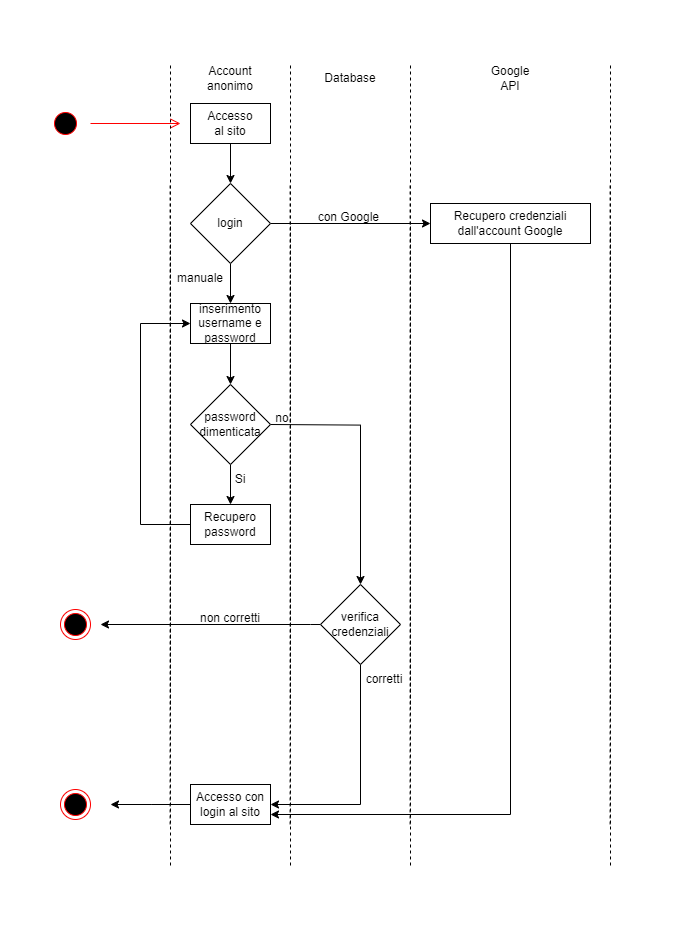
\includegraphics[width=1\textwidth]{img-D2/diagramma_login.png}
    \caption{ Diagramma attività login}
\end{figure}

\subsubsection*{RF8 Ricerca}
\begin{figure}[H]
   \centering
   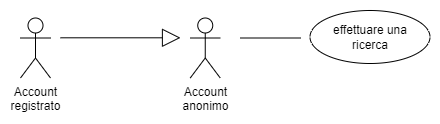
\includegraphics[width=0.7\textwidth]{img-D2/ricerca.png}
    \caption{USE-CASE Ricerca}
\end{figure}

\subsubsection*{RF7.1 Visualizza recensioni, RF9 Visualizzare montagne-rifugi}
\begin{figure}[H]
   \centering
   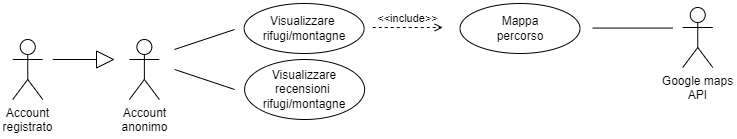
\includegraphics[width=1.0\textwidth]{img-D2/visualizzare_montagne.png}
    \caption{USE-CASE Visualizza Montagne-Rifugi-Recensioni}
\end{figure}


\subsubsection*{RF11 Supporto}
\begin{figure}[H]
   \centering
   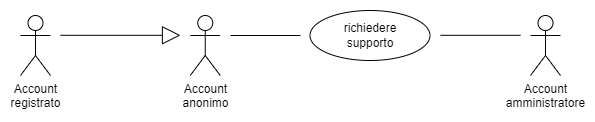
\includegraphics[width=1\textwidth]{img-D2/richiesta_supporto.png}
    \caption{USE-CASE Richiesta supporto}
\end{figure}

\subsubsection*{RF12 Cambio lingua}
\begin{figure}[H]
   \centering
   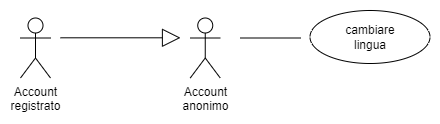
\includegraphics[width=0.8\textwidth]{img-D2/cambio_lingua.png}
    \caption{USE-CASE Cambio lingua}
\end{figure}

\subsubsection*{RF13 Meteo della Montagna}
\begin{figure}[H]
   \centering
   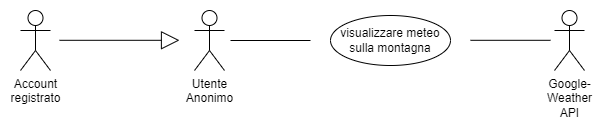
\includegraphics[width=1\textwidth]{img-D2/meteo.png}
    \caption{USE-CASE Meteo montagna}
\end{figure}


\subsection*{RF3 Account Amministratore}
\subsubsection*{RF2 Login amministratore}
\begin{figure}[H]
   \centering
   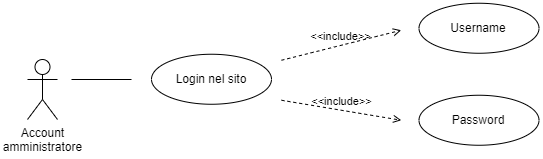
\includegraphics[width=0.8\textwidth]{img-D2/login_amministratore.png}
    \caption{USE-CASE Login}
\end{figure}

\subsubsection*{RF3.1 Eliminare utenti registrati}
\begin{figure}[H]
   \centering
   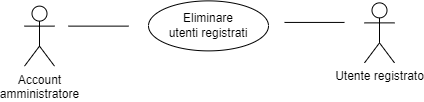
\includegraphics[width=0.6\textwidth]{img-D2/eliminazione_utenti.png}
    \caption{USE-CASE Eliminazione utenti}
\end{figure}

\subsubsection*{RF3.2 Eliminare recensioni}
\begin{figure}[H]
   \centering
   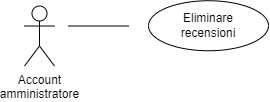
\includegraphics[width=0.4\textwidth]{img-D2/eliminazione_recensioni.png}
    \caption{USE-CASE Eliminazione recensioni}
\end{figure}

\subsubsection*{RF3.3 Modificare/Eliminare montagna o rifugio}
\begin{figure}[H]
   \centering
   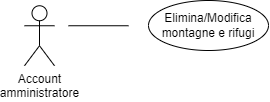
\includegraphics[width=0.4\textwidth]{img-D2/m_e_montagna_rifugio.png}
    \caption{USE-CASE Modifica/Eliminazione montagne e/o rifugi}
\end{figure}

\subsubsection*{RF3.4 Rispondere alle richieste di supporto}

\begin{figure}[H]
   \centering
   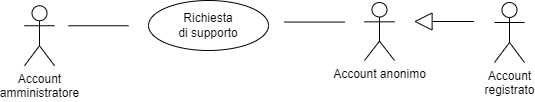
\includegraphics[width=0.8\textwidth]{img-D2/richiesta_supporto_amministratore.png}
    \caption{USE-CASE Risposta alla richiesta di supporto}
\end{figure}




\subsection*{RF4 Account registrato}

Di seguito vengono descritte le funzioni dell'account registrato.

\subsubsection*{RF7 Recensioni}
\begin{figure}[H]
   \centering
   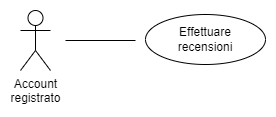
\includegraphics[width=0.4\textwidth]{img-D2/recensioni_registrato.png}
    \caption{USE-CASE Recensioni}
\end{figure}
 
\subsection*{RF6 Profilo utente}
\begin{figure}[H]
   \centering   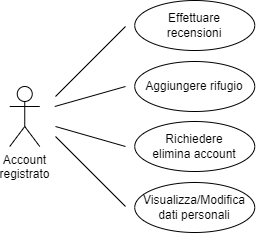
\includegraphics[width=0.3\textwidth]{img-D2/profilo_utente.png}
    \caption{USE-CASE Profilo utente}
\end{figure}


\subsection*{Use case totale}
\begin{figure}[H]
   \centering
    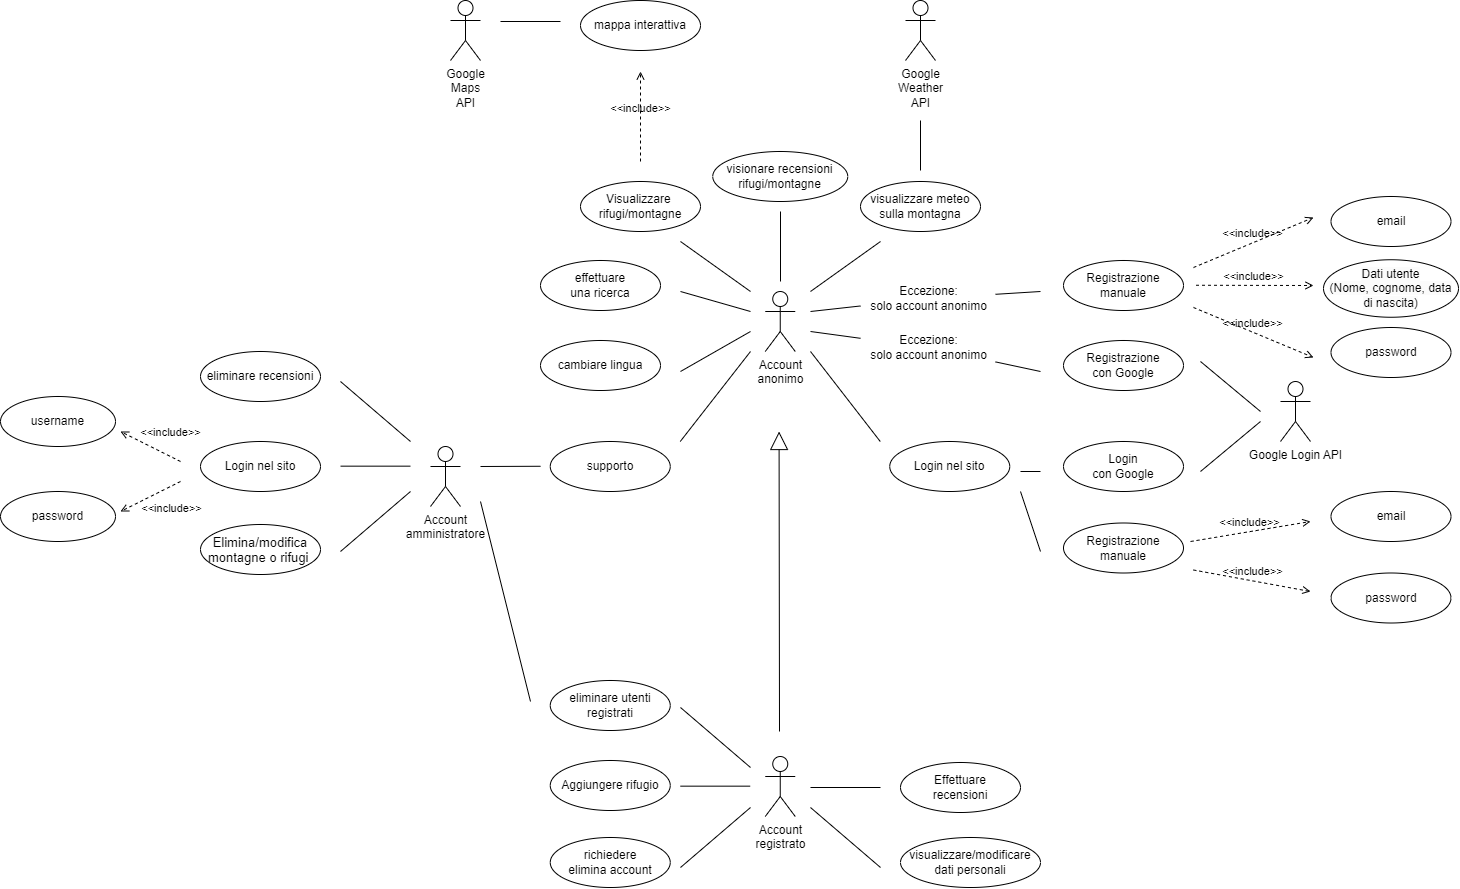
\includegraphics[width=1\textwidth]{img-D2/use_case_completo.png}
    
\end{figure}
Eccezioni:
\begin{itemize}
    \item La registrazione manuale la può fare solo un utente anonimo
    \item La registrazione con Google la può fare solo un utente anonimo
\end{itemize}{}



{\newpage}
\section{Requisiti non funzionali}

Vengono di seguito elencati e descritti i requisiti non funzionali del progetto. Ciascun requisito diversamente dai requisiti funzionali è legato alle performance.\\
Per ogni requisito funzionale, viene fatta una descrizione a cui viene accompagnata una misura, per poter verificare se il requisito funzionale è stato soddisfatto o meno.

\subsection*{RNF1 Sicurezza}

\begin{table}[H]
    \centering
    \begin{tabular}{|p{0.2\textwidth}|p{0.38\textwidth}|p{0.38\textwidth}|}
    

        \hline 
         Proprietà & Descrizione & Misura\\
         \hline      
         
         Password sicure&  Gli utenti associano un username al proprio account e una password sicura che permette la protezione dei propri dati personali& Una password sicura deve avere una lunghezza minima di 8 caratteri, lettere sia maiuscole che minuscole, inoltre devono essere presenti almeno un carattere speciale (\&, £, \$, \#, ...) e almeno un numero.\\ \hline
        Utilizzo TLS/SSL & Tutti i dati sensibili degli utenti, come informazioni personali e password, saranno crittografati sia in transito, sia quando il dato non viene utilizzato
        per l’accesso & Il link della pagina deve contenere https all'inizio di esso, ossia un protocollo per la comunicazione sicura attraverso Internet. La trasmissione verrà effettuata sulla porta 443 (standard per l'https). \\  \hline
        Email verificata & L’indirizzo email inserito dall’utente deve essere verificato &
        Quando l'utente effettua la registrazione, oppure elimina il proprio account, un'email di verifica viene inviata per confermare l'identità.
        \\ \hline
    \end{tabular}

    \caption{Sicurezza}
\end{table}

\subsection*{RNF2 Performance}

\begin{table}[H]
    \centering
    \begin{tabular}{|>{\centering}p{0.2\textwidth}|p{0.38\textwidth}|p{0.38\textwidth}|}
        \hline  
         Proprietà & Descrizione & Misura\\
         \hline      
         Performance  
         &Il sito deve essere in grado di gestire il numero richiesto di utenti senza alcun degrado delle prestazioni. Deve essere inoltre veloce e rendere gradibile la navigazione.
         &  Le performance vengono stabilite da il tempo di risposta dopo un’operazione dell’utente, per garantire alte performance il tempo massimo di rispsota sarà di 2 secondi.\\ \hline
    \end{tabular}
    \caption{Performance}
    
\end{table}


\subsection*{RNF3 Compatibilità}
\begin{table}[H]
    \centering
    \begin{tabular}{|p{0.2\textwidth}|p{0.38\textwidth}|p{0.38\textwidth}|}
        
         \hline  
         Proprietà & Descrizione & Misura\\
         \hline
         Compatibilità
         & Gli utenti devono poter accedere al sito web tramite l'utilizzo di qualisiasi dispositivo,  tra computer, tablet e smartphone, utilizzando uno dei browser supportati.
         & Il sito web deve essere supportato nel 95\% dei dispositivi.\\ \hline
    \end{tabular}
    
    \caption{Compatibilità}
\end{table}


\subsection*{RNF4 Affidabilità e disponibilità}
\begin{table}[H]
    \centering
    \begin{tabular}{|p{0.2\textwidth}|p{0.38\textwidth}|p{0.38\textwidth}|}
         \hline  
         Proprietà & Descrizione & Misura\\
         \hline 
            Affidabilità
         &  i dati inseriti dagli utenti verranno salvati all’interno di un database. Su questi verranno effettuati backup, per poter eventualmente recuperare i dati in caso di guasti del sistema o di attacchi informatici.
         & I backup verranno eseguiti ogni 7 giorni.\\ \hline
         Disponibilità & La disponibilità del sito è la capacità di essere accessibile agli utenti in qualsiasi momento, Per garantire un'ottima disponibilità del sito sarà necessario un ottimo servizio di hosting con strutture ridondanti. & Il sito dovrà essere disponibile almeno 23 ore al giorno, 7 giorni a settimana. \\ \hline
    \end{tabular}
    \caption{Affidabilità e disponibilità}
\end{table}


\subsection*{RNF5 Usabilità}
\begin{table}[H]
    \centering
    \begin{tabular}{|p{0.2\textwidth}|p{0.38\textwidth}|p{0.38\textwidth}|}
        \hline  
         Proprietà & Descrizione & Misura\\
         \hline      
         Usabilità
         & Gli utenti devono essere in grado di saper utilizzare il sito web in maniera completa senza bisogno di dover utilizzare alcun manuale, in breve tempo.
         &Un utente deve essere in grado di utilizzare completamente il sito dopo 15 minuti.\\ \hline
    \end{tabular}
    \caption{Usabilità}
\end{table}


\subsection*{RNF6 Norme recensioni}
\begin{table}[H]
    \centering
    \begin{tabular}{|p{0.2\textwidth}|p{0.38\textwidth}|p{0.38\textwidth}|}
        \hline  
         Proprietà & Descrizione & Misura\\
         \hline      
         Norme recensioni
         & Le recensioni devono essere conformi a norme contro discriminazioni o blasfemie.
         &Le recensioni che conterranno discriminazioni o blasfemie verranno eliminate dall'account amministratore.\\ \hline
    \end{tabular}
    \caption{Norme recensioni}
\end{table}

\subsection*{RNF7 Gestione delle immagini}
\begin{table}[H]
    \centering
    \begin{tabular}{|p{0.2\textwidth}|p{0.38\textwidth}|p{0.38\textwidth}|}
        \hline  
         Proprietà & Descrizione & Misura\\
         \hline      
         Gestione immagini
         & Le immagini devono essere gestite in modo da non provocare un rallentamento del sito web.
         &La massima dimensione delle immagini caricate dagli utenti è di 3MB.\\ \hline
    \end{tabular}
    \caption{Gestione immagini}
\end{table}


\subsection*{RNF8 Privacy}
\begin{table}[H]
    \centering
    \begin{tabular}{|p{0.2\textwidth}|p{0.38\textwidth}|p{0.38\textwidth}|}
        \hline  
         Proprietà & Descrizione & Misura\\
         \hline      
         GDPR
         & Il sito raccoglierà e tratterà dati
        personali degli utenti, dopo aver fornito avvisi chiari sulla privacy e acquisito i consensi necessari.
         &Conforme\\ \hline
         Copyright
         & Sarà rispettato il copyright per tutti i contenuti utilizzati sul sito.
         &Sarà avitato l’uso non autorizzato di testi, immagini e altri materiali protetti.\\ \hline
         COPPA
         & Il sito effettuerà un controllo dell’età dell’utente che si registra.
         &L'utente che si registra deve avere minimo 13 anni.\\ \hline
    \end{tabular}
    \caption{Privacy}
\end{table}


\subsection*{RNF9 Aggiornamenti} 
\begin{table}[H]
    \centering
    \begin{tabular}{|p{0.2\textwidth}|p{0.38\textwidth}|p{0.38\textwidth}|}
        \hline  
         Proprietà & Descrizione & Misura\\
         \hline      
         Aggiornamenti
         & Il sito web sarà sviluppato con un'infrastruttura scalabile, per garantire l'aggiunta di nuove funzionalità e il miglioramento complessivo dell'esperienza utente.
         & Una volta al mese verrà effettuato un controllo sull'adeguatezza dell'architettura, e in caso verranno effettuati opportuni aggiornamenti.\\ \hline
    \end{tabular}
    \caption{Aggiornamenti}
\end{table}
 


\newpage

\section{Diagramma di contesto}
Il diagramma di contesto fornisce una visione chiara delle interazioni tra il sistema, gli utenti registrati e l'amministratore. 

\subsection{Descrizione}

\begin{enumerate}
    \item Attori: Ci sono tre attori principali identificati:
    \begin{itemize}
        \item Utente Anonimo (RF5)
        \item Amministratore (RF3)
        \item MountainsWonders (il sistema centrale)
        \item Mail Service
        \item Google login API 
        \item Database
    \end{itemize}
    
    \item Interazioni Utente Anonimo - MountainsWonders:  
    \begin{itemize}
        \item L'Utente Anonimo può registrarsi direttamente attraverso il sito o tramite Google.(RF1) 
        \item Può effettuare l'accesso sia usando le credenziali del sito sia tramite Google.(RF2)
        \item L'Utente Anonimo può richiedere il reset della password.
        \item Può effettuare ricerche e visualizzare montagne o rifugi basandosi sui risultati di tali ricerche. (RF8)
        \item Può richiedere supporto e ricevere una risposta. (RF11)
    \end{itemize}
    
    \item Interazioni Amministratore - MountainsWonders:
    \begin{itemize}
        \item L'Amministratore può effettuare l'accesso. (RF2)
        \item Può ricevere messaggi di richiesta di supporto e fornire risposte. (RF3.4)
    \end{itemize}
    
    \item Interazioni MountainsWonders - Database:
    \begin{itemize}
        \item Tramite le interazioni con il database il sito si occupa della registrazione, l'autenticazione, le ricerche e altre funzioni correlate. (RF1, RF2, RF8)
    \end{itemize}
    
    \item Interazioni MountainsWonders - Servizi Esterni:
    \begin{itemize}
        \item MountainsWonders comunica con un servizio di posta elettronica per inviare email.
        \item Utilizza Google Login API per gestire l'autenticazione tramite Google. (RF1, RF2)
    \end{itemize}
    
\end{enumerate}

\begin{figure}[H]
   \centering   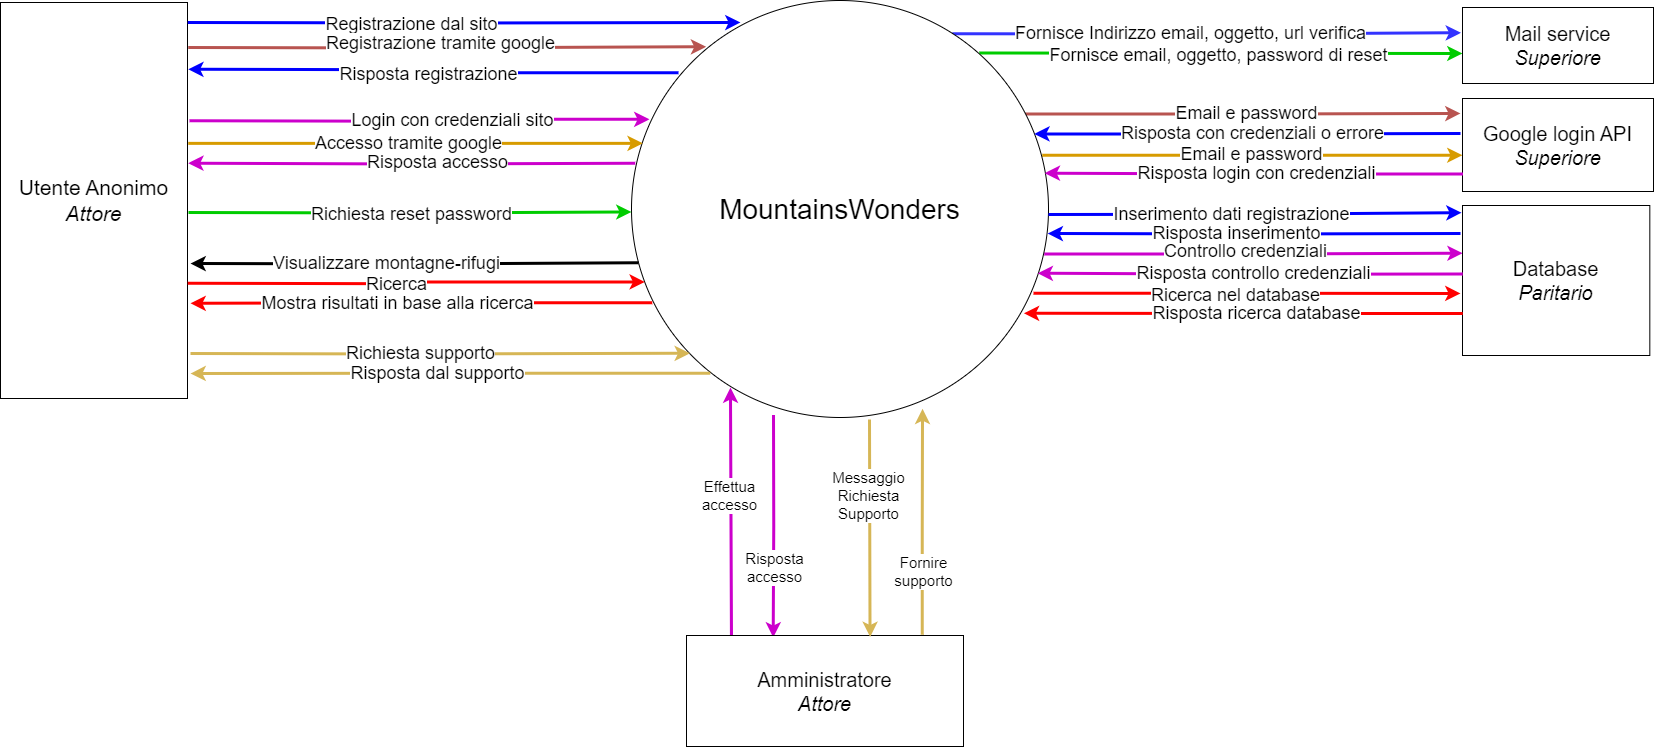
\includegraphics[width=1.0\textwidth]{img-D2/contesto_anonimo.png}
    \caption{Diagramma di contesto Utente Anonimo}
\end{figure}



\subsection{Descrizione}
Analizziamo il contenuto del secondo diagramma di contesto:




\begin{enumerate}
    \item Attori: Ci sono tre attori principali identificati:
    \begin{itemize}
        \item Utente Registrato (RF4)
        \item Amministratore (RF3)
        \item MountainsWonders (il sistema centrale)
    \end{itemize}


    
    \item Interazioni Utente Registrato - MountainsWonders:
    \begin{itemize}
        \item L'Utente Registrato può richiedere la visualizzazione dei propri dati personali e ricevere una risposta. (RF6)
        \item Ha la possibilità di modificare i propri dati personali e ricevere un feedback sulla modifica. (RF6) 
        \item Può inserire rifugi e ricevere una conferma sull'inserimento.
        \item Ha la possibilità di inserire o eliminare recensioni e ricevere un feedback su tali azioni. (RF7)
        \item Può visualizzare le recensioni effettuate. (RF6) 
        \item  Ha la possibilità di richiedere l'eliminazione del proprio account e ricevere una risposta in merito. (RF6)
    \end{itemize}

    
    \item Interazioni Amministratore - MountainsWonders:
    \begin{itemize}
        \item Può eliminare utenti (RF3.1)
        \item Elimina recensioni effettuate dagli utenti (RF3.2)
        \item Può ricevere messaggi di richiesta di supporto e fornire risposte. (RF3.4)
    \end{itemize}
    
    \item Interazioni MountainsWonders - Servizi Esterni:
    \begin{itemize}
        \item  MountainsWonders interagisce con il databse per propagre le operazioni fatte dall'utente e dall'amministratore.
        
    \end{itemize}
\end{enumerate}










\begin{figure}[H]
   \centering   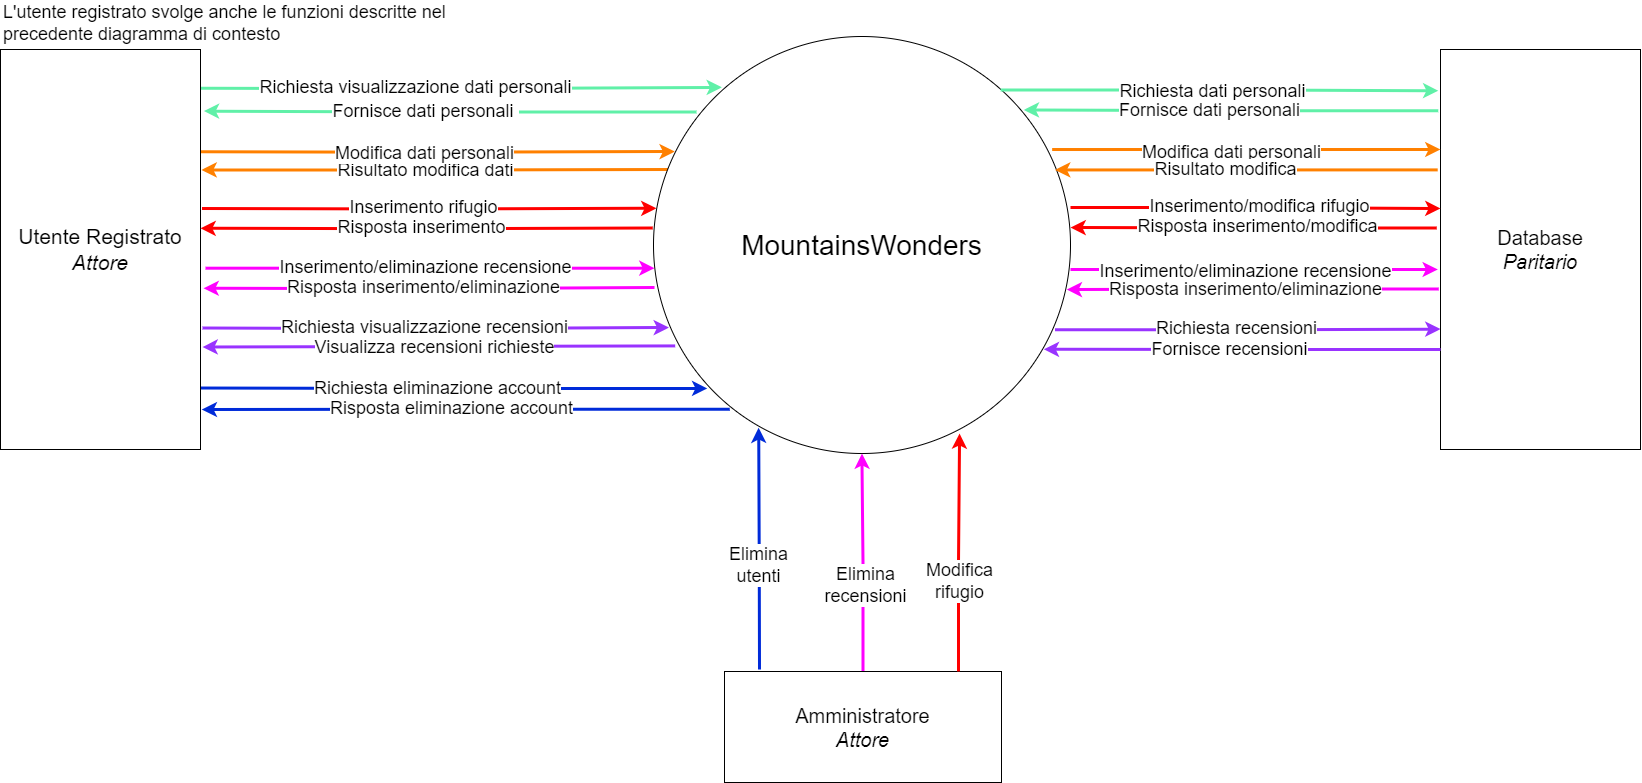
\includegraphics[width=1.0\textwidth]{img-D2/contesto_registrato.png}
    \caption{Diagramma di contesto Utente Registrato}
\end{figure}

\end{document}